%%% Preamble
\documentclass[paper=a4, fontsize=11pt]{report}

\usepackage[utf8]{inputenc}
\usepackage[T1]{fontenc}
\usepackage{fourier}
\usepackage[french]{babel}
\usepackage[protrusion=true,expansion=true]{microtype}	
\usepackage{amsmath,amsfonts,amsthm} % Math packages
\usepackage[pdftex]{graphicx}	
\usepackage{url}
\usepackage{pdfpages}
\usepackage{todonotes}
\usepackage[a4paper, body={16cm,23cm}]{geometry}
\usepackage{float}
\usepackage{framed}
\usepackage[toc,page]{appendix} 
\usepackage{multicol}
\usepackage{colortbl}

%%% Custom sectioning
\usepackage{sectsty}
\allsectionsfont{  \normalfont\scshape}
%\allsectionsfont{\centering \normalfont\scshape}

%%% Custom headers/footers (fancyhdr package)
\usepackage{fancyhdr}
\pagestyle{fancyplain}
\fancyhead{}								% No page header
\fancyfoot[L]{}							% Empty 
\fancyfoot[C]{}							% Empty
\fancyfoot[R]{\thepage}					% Pagenumbering
\renewcommand{\headrulewidth}{0pt}		% Remove header underlines
\renewcommand{\footrulewidth}{0pt}		% Remove footer underlines
\setlength{\headheight}{13.6pt}


%%% Equation and float numbering
\numberwithin{equation}{section}		% Equationnumbering: section.eq#
\numberwithin{figure}{section}		% Figurenumbering: section.fig#
\numberwithin{table}{section}		% Tablenumbering: section.tab#


%%% Define new commands
\newcommand{\horrule}[1]{\rule{\linewidth}{#1}} 	% Horizontal rule
\renewcommand{\bf}[1]{\textbf{#1}}
\renewcommand{\it}[1]{\textit{#1}}
\newcommand{\bfit}[1]{\textbf{\textit{#1}}}

\newcommand{\Todo}[1]{\todo[inline]{#1}}
\renewcommand{\thesection}{\thepart .\arabic{section}}

\usepackage{cases}
\usepackage{color}
\usepackage{xcolor}
\usepackage{relsize}

\usepackage{caption}
\DeclareCaptionFont{white}{\color{white}}
\DeclareCaptionFormat{listing}{\colorbox{gray}{\parbox{\textwidth}{#1#2#3}}}
\captionsetup[lstlisting]{format=listing,labelfont=white,textfont=white}

\usepackage[numbered]{mcode}

\lstset{breaklines=true,columns=fullflexible}
\colorlet{shadecolor}{black!10}

\delimitershortfall-1sp
\newcommand\abs[1]{\left|#1\right|}

%%% Begin document
\begin{document}

\includepdf[pages={1}]{title.pdf}

\tableofcontents

\listoftodos

\newpage

%%%%%%%%%%%%%%%%%%%%%%%%%%%%%%%%%%%%%%%%%%%%%%%%%%%%%%%%%%%%%%%%%%%%%%%%%%%%%%%%%%%%%%%%%%%%%%%%%%%%%%%%%%%%%%%%%%%%%%%%%%%
%%%%%%%%%%%%%%%%%%%%%%%%%%%%%%%%%%%%%%%%%%%%%%%%%%%%%%%%%%%%%%%%%%%%%%%%%%%%%%%%%%%%%%%%%%%%%%%%%%%%%%%%%%%%%%%%%%%%%%%%%%%
%%%%%%%%%%%%%%%%%%%%%%%%%%%%%%%%%%%%%%%%%%%%%%%%%%%%%%%%%%%%%%%%%%%%%%%%%%%%%%%%%%%%%%%%%%%%%%%%%%%%%%%%%%%%%%%%%%%%%%%%%%%
\part{Introduction}
\label{part:introduction}

\section{Présentation du contenu du rapport}
\label{sec:presentation-du-contenu-du-rapport}

Ce document constitue la synthèse de l'ensemble des livrables devant être remis à la fin du projet Développement Orienté Objet effectué en 4IF. Il a été convenu avec les professeurs encadrant le projet que le code pouvait être réalisé en langue anglaise mais que ceci impliquait également le rendu de certains livrables en Anglais. Les livrables devant être rendu en Anglais ont été identifiés avec les professeurs lors de la première séance de TP. Il sera donc indiqué dans le titre de chaque partie si le contenu de la partie est rédigé en Anglais \it{(EN)} ou en Français \it{(FR)}.  

%%%%%%%%%%%%%%%%%%%%%%%%%%%%%%%%%%%%%%%%% Capture et analyse des besoins

\part{Capture et analyse des besoins}
\label{part:capture-et-analyse-des-besoins}

\section{Planning prévisionnel du projet \it{(FR)}}
\label{sec:planning-previsionnel-du-projet}

\begin{figure}[H]
\centering
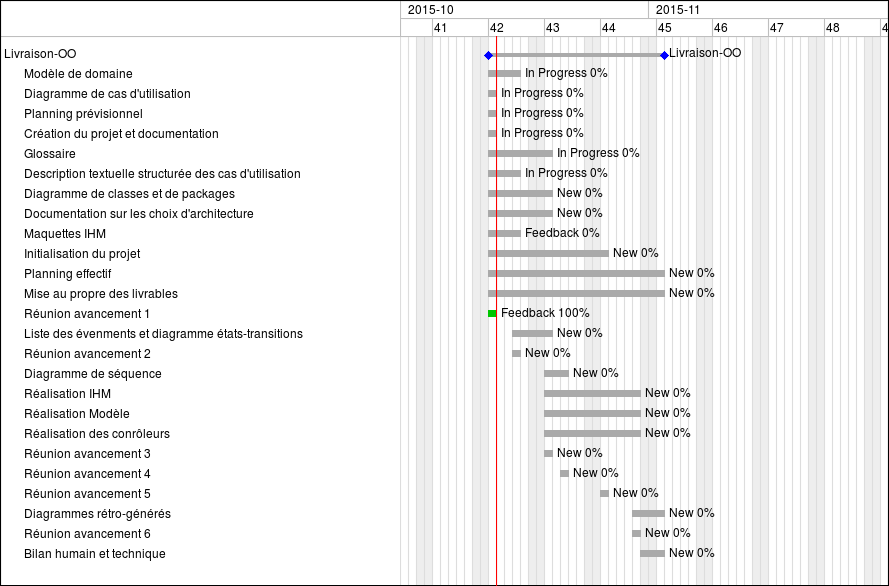
\includegraphics[scale=0.5,angle=0]{figures/gantt-prev.png}
\caption{Planning prévisionnel}
\end{figure}

\Todo{Ajouter tableau déroulement et affectation des tâches}

\section{Domain model \it{(EN)}}
\label{sec:domain-model}

\Todo{We should add a comment here}

\begin{figure}[H]
\centering
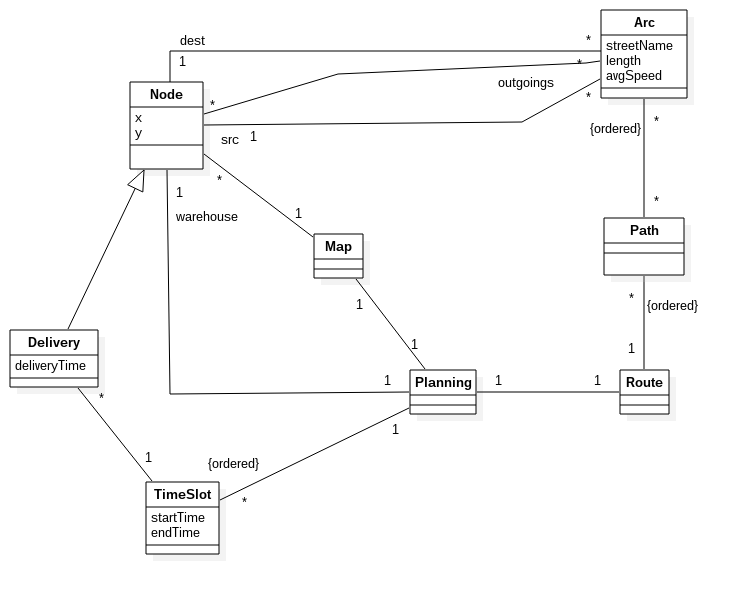
\includegraphics[scale=0.5,angle=0]{figures/domain-model.png}
\caption{Domain Model}
\end{figure}

\section{Glossary \it{(EN)}}
\label{sec:glossary}

Syntax used :
\begin{itemize}
	\item[\textbullet] \bf{Object} \it{(french equivalent)} : definition \\
\end{itemize}

Glossary : 
\begin{itemize}
	\item[\textbullet] \bf{Arc} \it{(tronçon)} : section of road between two intersections described by a street name, an average speed, a length and the id of the destination intersection.
	\item[\textbullet] \bf{Node} \it{(intersection)} : Intersection between two or more arcs (cf. Arc) described by its coordinates and an id.
	\item[\textbullet] \bf{Path} \it{(chemin)} : Ordered list of arcs between two delivery nodes, representing the shortest travel duration.
	\item[\textbullet] \bf{Map} \it{(plan)} : Set of arcs (cf. Arc) and intersections (cf. Node)
	\item[\textbullet] \bf{Delivery} \it{(livraison)} : Special node which must be contained by the final route.
	\item[\textbullet] \bf{Planning} : Set of intersections (cf. Node) to be processed by the route computation algorithm (cf. Route).
	\item[\textbullet] \bf{Route} \it{(tournée)} : Ordered list of paths to travel along (cf. Planning). 
	\item[\textbullet] \bf{TimeSlot} \it{(fenêtre de livraison)} : time interval bounded by a start time and an end time containing a set of deliveries to be honored.
	\item[\textbullet] \bf{Warehouse} \it{(entrepot)} : Special intersection representing both the start and the end point of the route (cf. Route).
	\item[\textbullet] \bf{Average Speed} \it{(vitesse moyenne)} : average speed of vehicles in meters per second on an arc (cf. Arc).
	\item[\textbullet] \bf{Planning File} \it{(fichier de planning)} : XML formated input file, describing a planning (cf. Planning).
	\item[\textbullet] \bf{Map File} \it{(fichier de plan)} : XML formated input file, describing a Map.
	\item[\textbullet] \bf{Route File} \it{(fichier d’itinéraire)} : text formated output file, describing paths to travel along.
\end{itemize}

\section{Use case diagram \it{(EN)}}
\label{sec:use-case-diagram}

\Todo{We should add a comment here}

\begin{figure}[H]
\centering
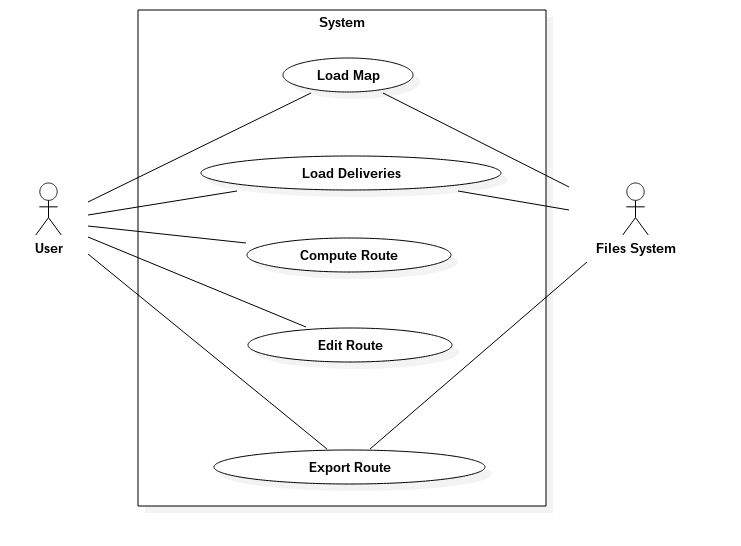
\includegraphics[scale=0.5,angle=0]{figures/use-case.png}
\caption{Use case diagram}
\end{figure}

\section{Structured textual description of use cases \it{(EN)}}
\label{sec:structured-textual-description-of-use-cases}

\subsection{Textual description of \bfit{Load map}}
\label{subsec:textual-description-of-load-map}

\textbf{Short description :} The user selects an XML file describing a city map. The map is loaded and displayed on the screen.

\textbf{Organized description :}

\begin{itemize}
  \item[•] \textbf{Precondition :} none.
  \item[•] \textbf{Main scenario :}
  \begin{enumerate}
    \item The user indicates that he wants to load a map
    \item The system opens a dialog box allowing the user to select a file.
    \item The user selects the XML file describing the map that he wants to load in the program.
    \item The system interprets the XML file, loads the city map and display the map on the screen.
    \item The user can’t cancel his former modifications anymore.
  \end{enumerate}
  \item[•] \textbf{Alternative scenarios :}
  \begin{itemize}
    \item[3a.] The users indicates that he wants to stop the selection of a city map.
    \begin{itemize}
      \item[•] Le system stops the selection and ends the scenario.
    \end{itemize}
    \item[4a.] The XML file selected is incorrect (cf. XML Errors Lists~\ref{subsec:xml-errors-lists}) and doesn’t define a city map.
    \begin{itemize}
      \item[•] The system indicates that the file is incorrect and can’t be loaded, and end the scenario.
    \end{itemize}
    \item[4b.] The opening and the reading of the XML file is denied (cf. IO Errors Lists~\ref{subsec:io-errors-list}).
    \begin{itemize}
      \item[•] The system displays that the loading has failed and indicates the cause (insufficient privileges…) and ends the scenario.
    \end{itemize}
  \end{itemize}
\end{itemize}

\Todo{Ajouter les autres scénarios à partir du drive}

%%%%%%%%%%%%%%%%%%%%%%%%%%%%%%%%%%%%%%%%%%%%%%%%%%%%%%%%%%%% Conception
\part{Conception}
\label{part:conception}

\section{User-level events list and State-Transition Diagram \it{(EN)}}
\label{sec:user-level-events-list-and-state-transition-diagram}

\begin{figure}[H]
\advance\leftskip-1cm
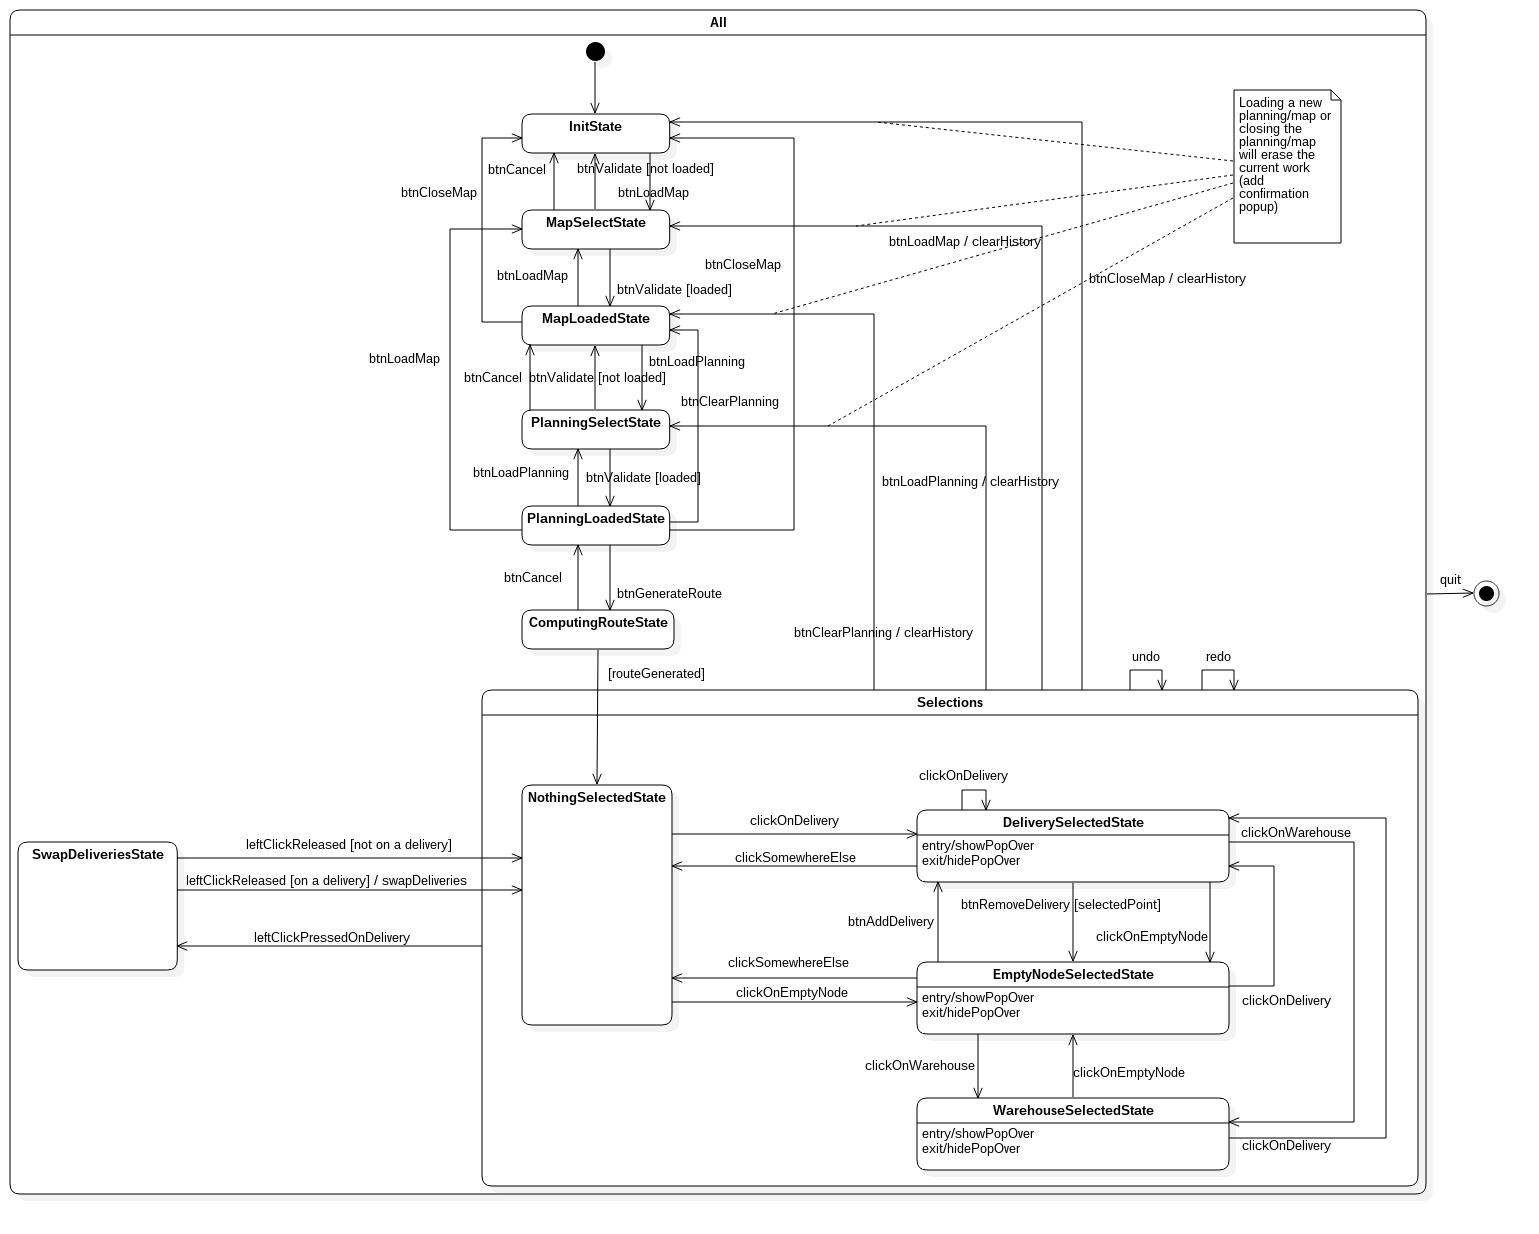
\includegraphics[scale=0.4,angle=90]{figures/state-machine.png}
\caption{State-Transition Diagram}
\end{figure}

\Todo{Add user-level events list}
\Todo{We should add a comment here}

\section{Packages and Classes Diagrams \it{(EN)}}
\label{sec:packages-and-classes-diagrams}

\subsection{Model related diagrams}
\label{subsec:model-related-diagrams}

\Todo{We should add a comment here}

\vspace*{-6cm}
\begin{figure}[H]
\centering
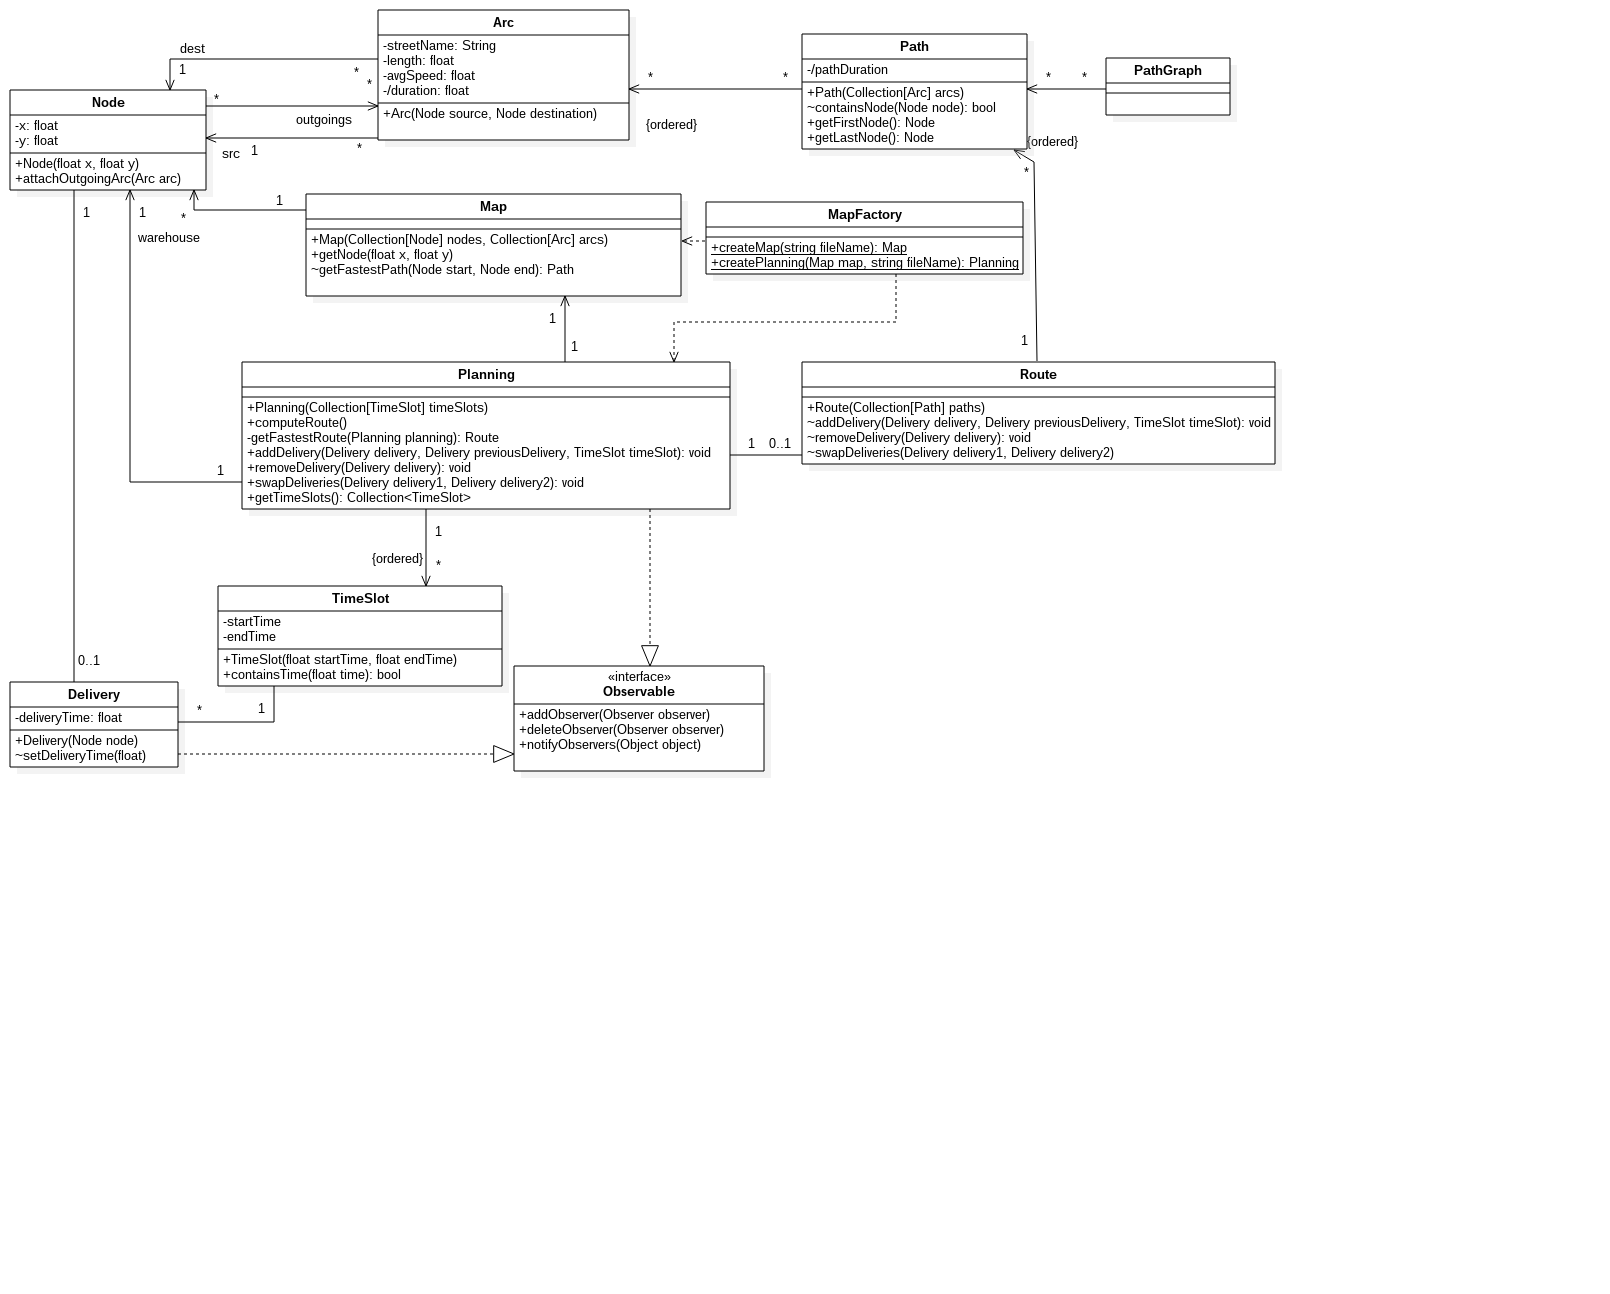
\includegraphics[scale=0.52,angle=90]{figures/model-class.png}
\caption{Model package including classes}
\end{figure}

\subsection{View related diagrams}
\label{subsec:view-related-diagrams}

\Todo{We should add a comment here}

\begin{figure}[H]
\advance\leftskip-1.5cm
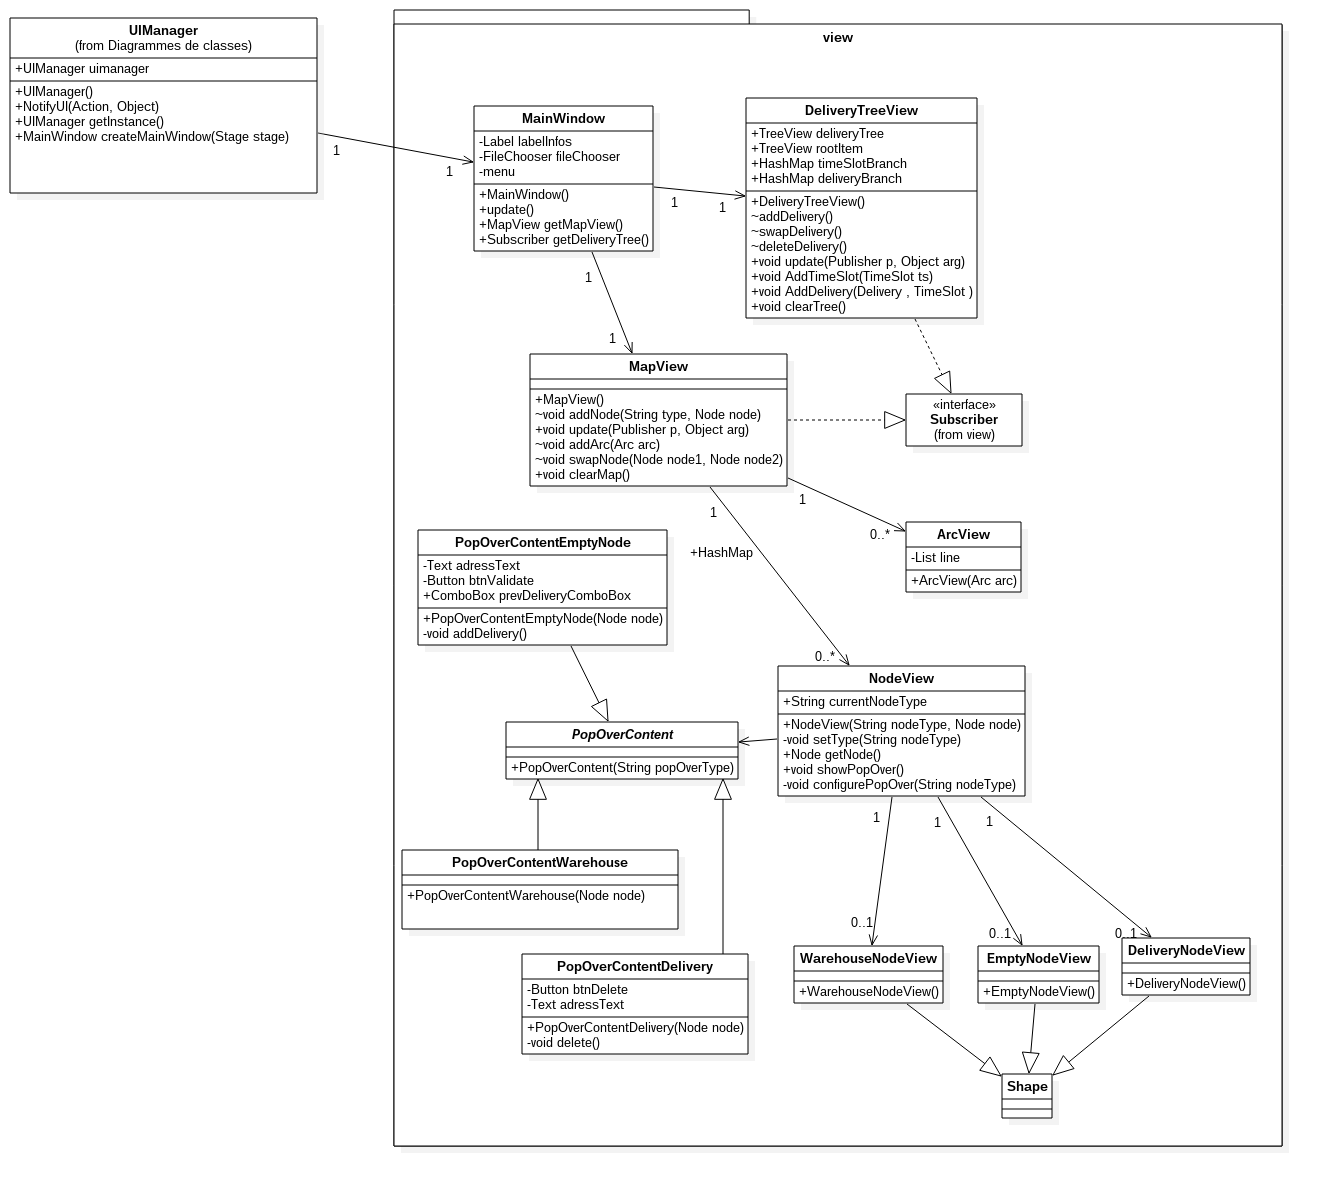
\includegraphics[scale=0.44,angle=0]{figures/view-class.png}
\caption{View package including classes}
\end{figure}

\subsection{Controller related diagrams}
\label{subsec:controller-related-diagrams}

\Todo{We should add a comment here}

\begin{figure}[H]
\centering
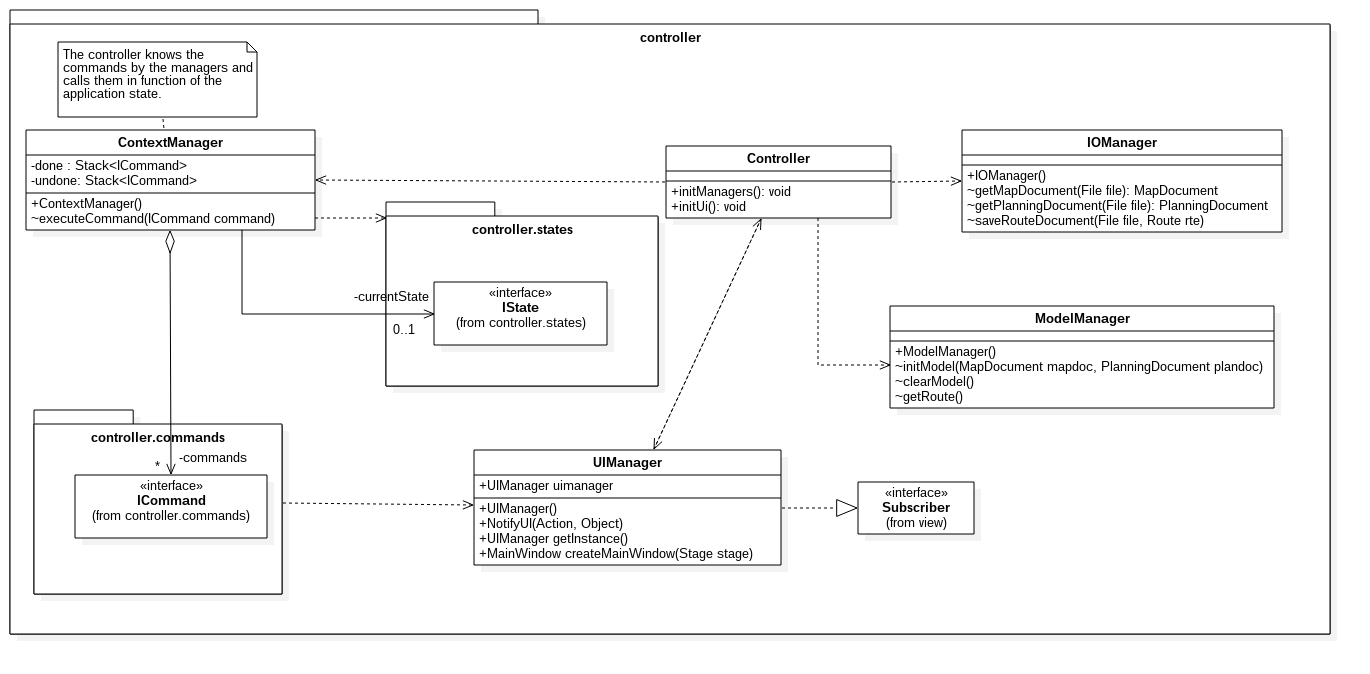
\includegraphics[scale=0.5,angle=90]{figures/controller-class.png}
\caption{Controller package including classes}
\end{figure}

\begin{figure}[H]
\advance\leftskip-1cm
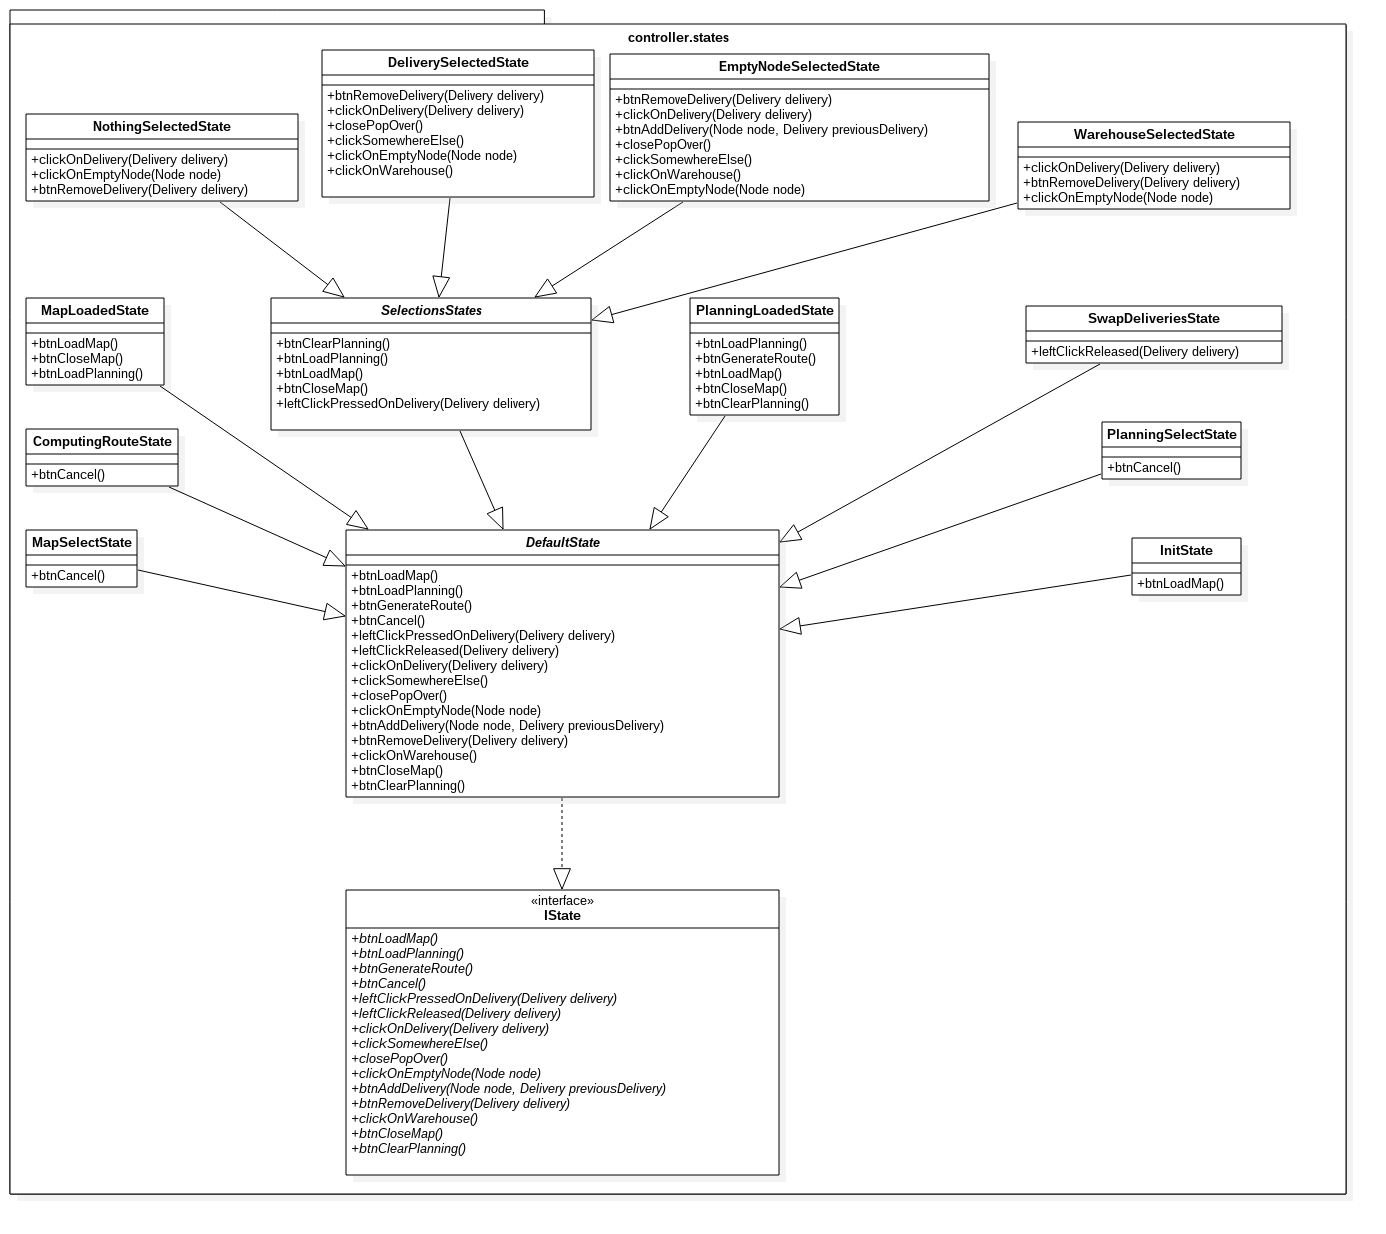
\includegraphics[scale=0.4,angle=0]{figures/controller_states-class.png}
\caption{Controller States package including classes}
\end{figure}

\begin{figure}[H]
\centering
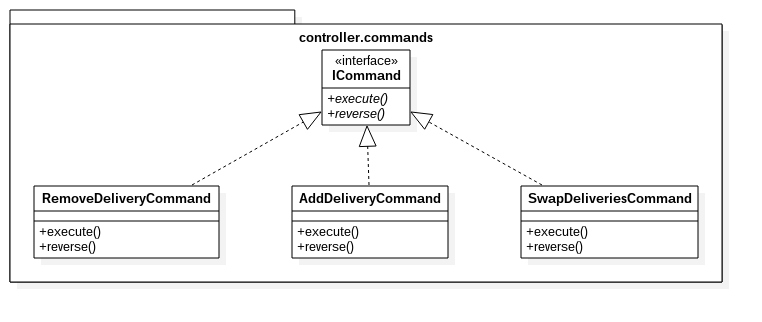
\includegraphics[scale=0.5,angle=0]{figures/controller_commands-class.png}
\caption{Controller Commands package including classes}
\end{figure}

\subsection{Other diagrams}
\label{subsec:other-diagrams}

\Todo{We should add a comment here}

\begin{figure}[H]
\centering
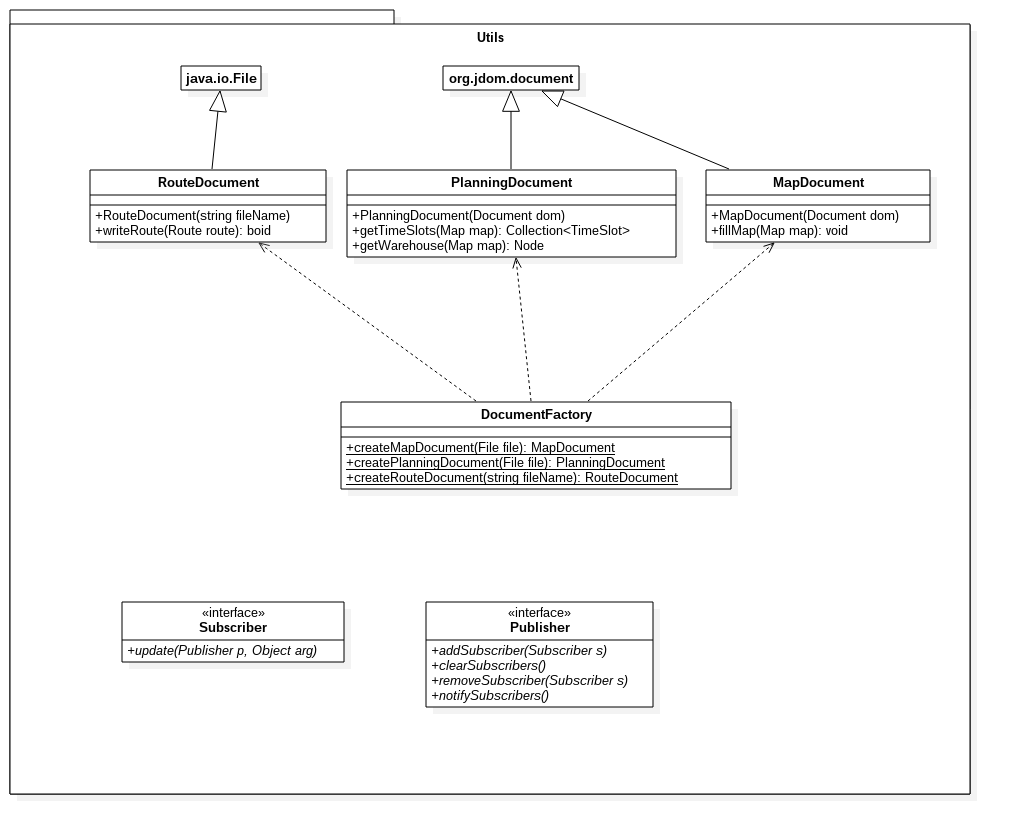
\includegraphics[scale=0.5,angle=0]{figures/utils-class.png}
\caption{Utils package and its classes}
\end{figure}

\section{Choix architecturaux et patrons de conception utilisés \it{(FR)}}
\label{sec:choix-architecturaux-et-patrons-de-conception-utilises}

\bfit{Les classes cités dans ce document pouvant présenter des ambiguïtés sont référencés dans le glossaire.} \\

Nous choisirons tout d'abord de respecter l'architecture globale de type \bf{MVC} afin de garantir une simplicité de maintenance corrective et évolutive de l'application. Les différents composants appartenant à ces trois grandes catégories (Modèle, Vue et Contrôleur) implémenteront divers patrons de conception. \\

Concernant l'architecture globale, nous avons choisi de faire en sorte que la hiérarchie en couche soit parfaitement respectée, c'est-à-dire que la vue ne modifie en aucun cas le modèle sans  passer par le contrôleur. La vue, cependant, implémente pour certains de ses composants le patron \bf{Observateur} pour détecter les modifications au niveau du modèle et se modifier ou demander au contrôleur d'effectuer des actions en conséquence.\\

Les objets du modèle, qui constitue l'ensemble des données métier manipulées par l'application représentées par des objets, sont pour la plupart des conteneurs de données améliorés et n'implémentent pas de traitements particuliers. Il y a cependant une exception, l'objet \bf{Map} implémente l'algorithme permettant de calculer la tournée et de créer l'objet \bf{Route} correspondant. Certains objets, tels que \bf{Map} et \bf{Planning}, constituent en réalité des conteneurs d'autres objets du modèle. Ces objets agissent comme des \bf{Fabrique}s pour les objets qu'ils contiennent. Cela permet de garantir la cohérence des objets contenus dans ces conteneurs ainsi que la maîtrise de la durée de vie de ces derniers. Comme indiqué dans le paragraphe précédent, le modèle est observé par la vue ce qui signifie que certains objets du modèle sont \bf{Observable}s. Ce mécanisme nous permet de notifier la vue de changements au niveau du modèle. \\

L'objet qui représente la \bf{Map}, \bf{MapView}, ainsi que celui qui représente l'arbre des livraisons implémentent le patron \bf{Observateur}. Pour le reste, la vue est isolée du modèle. Celui peut donc fonctionner indépendamment de la vue.\\

Nous avons ajouté un package supplémentaire n'apparaissant pas dans l'architecture MVC afin d'y placer tous les objets étant catégorisés utilitaires, c'est-à-dire rendant des services aux autres objets de l'application mais dont les traitements auraient pu être intégrés aux objets de l'application si nous n'avions pas fait le choix de segmenter les traitements. Ce package, nommé utils, contient notamment les objets constituant des interfaces plus simples pour la création des objets du modèle possédant une représentation sous forme de fichiers XML. Ce package contient également une classe permettant la conversion de types spéciaux propres à l'application et une \bf{Fabrique} pour les objets d'interface avec les fichiers. \\

Le choix majeur effectué concernant le contrôleur est de séparer les traitements en créant des sous-composants de ce contrôleur principal. Ce package contient donc un ensemble de  contrôleurs spécialisés. Cette organisation au niveau du contrôleur présente de nombreux avantages et notamment la simplification des procédures de gestion des erreurs, leurs causes étant segmentées à l'image des contrôleurs qui peuvent les rencontrer. 
Nous avons donc choisi de dédier un contrôleur à la gestion du modèle, il constitue en réalité l'interface du contrôleur avec le modèle. Ce contrôleur se nomme \bf{ModelManager} et garantie la cohérence du modèle exploité par l'application, tout en proposant une interface simple pour l'accès au modèle. Il ajoute également un niveau d'encapsulation supplémentaire concernant les données manipulées dans le modèle. 

Un second contrôleur, nommé \bf{IOManager}, est chargé des interactions avec le système de fichiers du système d'exploitation exécutant l'application. C’est à son niveau que sont traitées les erreurs de type Entrée/Sortie telles que l'absence de fichier ou encore les privilèges insuffisants pour lire/écrire un fichier. De nouveau, ce contrôleur propose une interface simple pour effectuer les opérations dont il est chargé. 

Ensuite, l'\bf{UIManager}, pendant du \bf{ModelManager}, mais pour l'interface graphique cette fois. Il constitue une interface, simple d'utilisation, entre le contrôleur et la vue. Cela permet de centraliser les informations provenant de la vue. C'est aussi le rôle de ce contrôleur d'interpréter les ordres en provenance de la vue pour les convertir en ordres exécutables par le \bf{ContextManager}. 

Le \bf{ContextManager} a deux rôles majeurs qui lui valent d'implémenter deux patrons de conception qui sont le patron État et le patron Commande. Il a tout d'abord pour rôle d'entretenir la machine à états globale de l'application, c'est-à-dire de garantir à chaque instant qu'une commande utilisateur déclenchera les bons traitements dans l'application et donc les bonnes réactions de l'interface utilisateur et du modèle. Son second rôle est d'entretenir un historique des modifications effectuées de sorte à ce que l'utilisateur puisse défaire et refaire les dernières actions qu'il a effectué. Ce contrôleur assure à l'utilisateur que l'action qu'il veut effectuer a du sens dans le processus global que déroule l'application. Il est dans cette optique étroitement lié à l'\bf{UIManager} qui lui fait parvenir les commandes de l'utilisateur.
Il est, à ce stade, important de préciser que ces différents composants implémentent tous le patron Singleton afin de garantir l'unicité de chaque interface et par conséquent l'unicité du modèle, de l'état de global de l'application et de l'historique des commandes effectuées.

L'objet \bf{Controller} présent dans le package ne constituent en réalité que le point d'entrée de l'application, il est appelé par la procédure main qui l'utilise pour initialiser les différents composants du contrôleur, c'est-à-dire réaliser la première instanciation des composants du contrôleur, puis démarrer l'interface graphique.

On peut également considérer l'\bf{UIManager} et le \bf{ModelManager} comme des \bf{Façade}s respectivement pour la vue et le modèle. 

\Todo{Ajouter des explications concernant les patrons de conception utilisés.}

\section{Sequence Diagram describing Route computation process \it{(EN)}}
\label{sec:sequence-diagram-describing-route-computation-process}

\Todo{Add sequence diagram here}

%%%%%%%%%%%%%%%%%%%%%%%%%%%%%%%%%%%%%%%%%%%%%%% Implémentation et tests

\part{Implémentation et tests}
\label{part:implementation-et-tests}

\section{Notes related to source code, its documentation and unit tests \it{(EN)}}
\label{sec:notes-related-to-source-code}

\Todo{Add notes here if needed or remove this section}

\section{Packages and classes diagrams generated from source code \it{(EN)}}
\label{sec:packages-and-classes-diagrams-generated-from-source-code}

\Todo{Retro-generated diagrams}

%%%%%%%%%%%%%%%%%%%%%%%%%%%%%%%%%%%%%%%%%%%%%%%%%%%%%%%%%%%%%%%% Bilan

\part{Bilan}
\label{part:bilan}

\section{Planning effectif du projet \it{(FR)}}
\label{sec:planning(effectif-du-projet}

\Todo{Ajouter le planning effectif (Gantt réel)}

\section{Bilan humain et technique \it{(FR)}}
\label{sec:bilan-humain-et-technique}

\Todo{Rédiger le bilan ici}

%%%%%%%%%%%%%%%%%%%%%%%%%%%%%%%%%%%%%%%%%%%%%%%%%%%%%%%%%%%%%%%% Annexes

\part{Annexes}
\label{part:annexes}

\section{Errors lists \it{(EN)}}
\label{sec:errors-lists}

\Todo{Expliquer ce que sont ces listes d'erreurs}

\subsection{IO Errors List}
\label{subsec:io-errors-list}

\textbf{Input errors :}
\begin{itemize}
  \item[•] \textbf{Cant Read File Error :} the folder is not readable, user’s privileges doesn’t match required privileges.
  \item[•] \textbf{Missing File Error :} the file is missing in file system. 
\end{itemize}

\textbf{Output errors :}
\begin{itemize}
  \item[•] Cant Write File Error : the folder is not readable, user’s privileges doesn’t match required privileges.  
\end{itemize}

\subsection{XML errors list}
\label{subsec:xml-errors-lists}

\textbf{Shared errors:}
\begin{itemize}
  \item[•] \textbf{Syntax errors :}
  \begin{itemize}
    \item[•] \textbf{Unexpected End Of File Error :} XML file is not well formatted, tags are not closed properly.
  \end{itemize}
\end{itemize}

\textbf{File specific errors :}
\begin{itemize}
  \item[•] \textbf{Semantic errors :}
  \begin{itemize}
    \item[•] \textbf{Map file :}
    \begin{itemize}
      \item[•] \textbf{Empty Map Error :} root tag has no child.
      \item[•] \textbf{Missing Node Attribute :} missing id, x or y attribute.
      \item[•] \textbf{Empty Node Error :} tag Node has no outgoing arc.
      \item[•] \textbf{Duplicate Node ID Error :} two or more nodes have the same ID.
      \item[•] \textbf{Duplicate Node Error :} two or more nodes have the same coordinates.
      \item[•] \textbf{Duplicate Arc Error :} two or more outgoing arcs of a single node have the same destination node. 
      \item[•] \textbf{Missing Destination Node Error :} the node referenced by an arc as its destination doesn’t exist. 
      \item[•] \textbf{Invalid Average Speed Value Error :} an arc specified average speed is missing, negative or zero. 
      \item[•] \textbf{Invalid Length Value Error :} an arc specified length is missing, negative or zero.
    \end{itemize}

    \item[•] \textbf{Planning file :}
    \begin{itemize}
      \item[•] \textbf{Missing Warehouse Error :} warehouse tag is missing or the id of the specified warehouse doesn’t match any of the node in the Map.
      \item[•] \textbf{Duplicate Warehouse Error :} more than one warehouse tag is present in the input file.
      \item[•] \textbf{Missing TimeSlot Error :} the file doesn’t specify a timeslot.
      \item[•] \textbf{Duplicate TimeSlot Error :} two or more timeslots have the same start time and end time.
      \item[•] \textbf{Null TimeSlot Error :} a timeslot has the same start and end time.
      \item[•] \textbf{Intersecting TimeSlot Error :} two or more timeslots are intersecting.
      \item[•] \textbf{Missing Delivery Node Error :} the address specified by a delivery doesn’t match any node in the Map.
      \item[•] \textbf{Duplicate Delivery Error :} two or more deliveries share the same destination. 
    \end{itemize}
  \end{itemize}
\end{itemize}

%%% End document
\end{document}
